\newcommand{\CloudMedianError}{0.076}
\newcommand{\CloudMaxError}{0.984}
\newcommand{\RelativeMedianError}{0.090}
\newcommand{\RelativeMaxError}{0.761}
\newcommand{\ControlCloudMaxError}{2.122}

\title{Self-Interacting Stochastic Dynamics with Exponential Memory:
An Observable-Matched Linear Relaxation Baseline}
\author{H. Horn}
\affiliation{Peine Stederdorf, Germany}
\date{9 October 2026}

\begin{abstract}
We study a stochastic trajectory coupled to a spatial trace with exponential
forgetting. A compact trace moving with the trajectory can resemble
self-localization even when its size is controlled by linear feedback.
We distinguish the current position relative to the trace centroid from the
width of the trace itself and derive their separate stationary second
moments. For a finite history, an impulse-response calculation and an
independent spectral integral give matching linear references without fitted
parameters. Reanalysis of nine active long-run slices, with five seeds each,
dimensions $d=3$--$20$, and runs up to $3\times10^8$ updates, gives a median
memory-cloud radius discrepancy of $\CloudMedianError\%$ and a maximum of
$\CloudMaxError\%$ in the stored terminal windows. Curvature-matched one-
and two-scale Gaussian kernels yield nearly identical scalar observables in
the small-radius regime. A separate fixed-gain test gives a smooth $6.24\%$
radius correction as the sampled scale increases, without resolving a
metastable transition. These results establish an observable-specific
baseline for the tested branch and delimit what compact memory clouds can
identify about the interaction kernel.
\end{abstract}
\maketitle

\section{Introduction}
Motion influenced by its own history occurs in reinforced walks, Brownian
polymers, and self-interacting diffusions
\cite{Pemantle2007,DurrettRogers1992}.
For normalized cumulative occupation measures, Bena\"im, Ledoux, and Raimond
developed a diffusion framework; symmetric interactions can drive the
occupation measure toward the critical set of a nonlinear free-energy
functional \cite{BenAImRaimond2002,BenaimRaimond2005}.
Exponentially fading traces replace cumulative averaging by a fixed
persistence scale. Aging-weighted diffusions with linear history
interactions, including an exponential case, have been studied by
Mili\v{s}i\'c, Meunier, and Roux \cite{MilisicMeunierRoux2026}.

The physical architecture of self-deposition and subsequent field response
also has established precedents. Walking-droplet models couple a moving
source to its decaying wave field \cite{OzaRosalesBush2013}; autochemotaxis
couples stochastic motion to a chemical signal and distinguishes transient
self-localization from long-time transport \cite{Grima2005}.
Those models include physical field propagation or diffusion and, in the
droplet case, inertial motion. Here the dynamics is a discrete overdamped
map with a nonpropagating deposited trace and a prescribed interaction
kernel. Adding auxiliary state to represent memory is likewise an
established method \cite{Mori1965,JaganathanValani2025}.

The contribution is a quantitative diagnostic for this specific map.
We match the theoretical and measured radius observables, including finite
history and averaging conventions, then test the same fixed reference
against archived long runs and kernel controls. This distinction matters:
the instantaneous width of a trace is not the distance of its most recent
point from its centroid, and a median instantaneous width is not a
stationary root-mean-square (RMS) radius. Agreement between different
quantities can obscure model and measurement errors.

\section{Deposited-Trace Model}
On $\mathbb R^d$, let $\mu_n$ be a finite nonnegative memory measure and
$K$ a smooth translation-invariant interaction potential. We require finite
second moments and integrable $K$ and $\nabla K$ against the memory. We use
\begin{align}
x_{n+1}&=x_n-\eta\nabla\Phi_n(x_n)+\varepsilon\xi_n,
\label{eq:trajectory}\\
\Phi_n(x)&=\int K(x-y)\,\mu_n(dy),
\label{eq:potential}\\
\mu_{n+1}&=q\mu_n+\alpha\delta_{x_{n+1}},\qquad q=1-\alpha,
\label{eq:memory}
\end{align}
where $0<\alpha<1$, $\eta\geq0$, and the independent innovations satisfy
$\xi_n\sim\mathcal N(0,I_d)$. The gradient acts on the evaluation coordinate
$x$ in Eq.~(\ref{eq:potential}); integrating over $y$ does not remove this
dependence. A unit-mass initial memory preserves unit mass under
Eq.~(\ref{eq:memory}). A centered deposition profile can replace the point
measure, but every simulation reported here uses point deposition.

The untruncated augmented state $(x_n,\mu_n)$ is Markov: it determines the
next-state law given a fresh innovation. The visible coordinate generally
fails this property because the same position with a different memory can
have a different drift. Exponential discounting supplies a persistence
scale $\alpha^{-1}$ updates. It need not destroy information in an exact
field representation, and we make no thermodynamic irreversibility claim.

The simulations retain the latest $H$ positions, with
\begin{equation}
\mu_n^H=\alpha\sum_{j=0}^{H-1}q^j\delta_{x_{n-j}},\qquad
M_H=1-q^H.
\label{eq:finite_memory}
\end{equation}
After the buffer fills, its mass is $M_H$, not one. The complete finite
Markov state is the ordered history buffer. The native update evaluates
the force first, advances $x$, deposits $x_{n+1}$, and retires the oldest
position. This convention fixes the timing in the comparisons below.

The kernel used in the long runs is
\begin{equation}
K(u)=A_r e^{-|u|^2/(2s_r^2)}-A_a e^{-|u|^2/(2s_a^2)}.
\label{eq:kernel}
\end{equation}
Its local restoring curvature is
$\kappa=A_a/s_a^2-A_r/s_r^2$. In a region where the pairwise separations are
small compared with the active kernel widths, the drift becomes
\begin{equation}
-\eta\nabla\Phi_n(x_n)\simeq-g(x_n-c_n),
\qquad g=\eta M\kappa,
\label{eq:linear_force}
\end{equation}
with $c_n$ the mass-normalized memory centroid and $M$ its mass.
This local approximation does not imply global confinement.

\section{Two Radius Observables}
For a normalized memory, define
\begin{equation}
r_n=x_n-c_n,\qquad
Q_n=\int |y-c_n|^2\,\mu_n(dy).
\label{eq:observables}
\end{equation}
The position-relative RMS is $R_r=\sqrt{\mathbb E|r_n|^2}$; the
memory-cloud RMS is $R_Q=\sqrt{\mathbb E Q_n}$. Their stationary
expectations concern the relative state, not a stationary absolute position.

\subsection{Untruncated reference}
For Eq.~(\ref{eq:memory}), the centroid obeys
$c_{n+1}=qc_n+\alpha x_{n+1}$. Substituting the linear force gives
\begin{equation}
r_{n+1}=q(1-g)r_n+q\varepsilon\xi_n.
\label{eq:relative_mode}
\end{equation}
If $|q(1-g)|<1$, the stationary position-relative second moment is
\begin{equation}
R_r^2=\frac{d q^2\varepsilon^2}{1-q^2(1-g)^2}.
\label{eq:position_radius}
\end{equation}
The variance of the deposited trace satisfies a different recursion:
\begin{equation}
Q_{n+1}=qQ_n+q\alpha|x_{n+1}-c_n|^2.
\label{eq:cloud_recursion}
\end{equation}
Since $r_{n+1}=q(x_{n+1}-c_n)$, stationarity gives
\begin{equation}
R_Q^2=R_r^2/q.
\label{eq:cloud_radius}
\end{equation}
The factor is small at $\alpha=0.01$, but the distinction remains exact.
Moreover, neither RMS equals the median of $\sqrt{Q_n}$.

\subsection{Finite-history reference}
The normalized weights are $w_j=\alpha q^j/M_H$. The exact finite
centroid update is
\begin{equation}
c_{n+1}^H=qc_n^H+\frac{\alpha}{M_H}
\left(x_{n+1}-q^H x_{n-H+1}\right).
\label{eq:finite_center}
\end{equation}
Replacing the mass in $g$ does not remove the retirement term. For the
linear map, define its normalized history filter and response denominator
on the unit circle by
\begin{align}
B_H(z)&=\sum_{j=0}^{H-1}w_jz^{-j},\\
F_H(z)&=1-z^{-1}+g z^{-1}[1-B_H(z)].
\label{eq:filter}
\end{align}
In the stationary relative regime the two matching second moments are
\begin{align}
R_{r,H}^2&=\frac{d\varepsilon^2}{2\pi}
\int_{-\pi}^{\pi}\frac{|1-B_H(e^{i\omega})|^2}
{|F_H(e^{i\omega})|^2}\,d\omega,\label{eq:finite_relative}\\
R_{Q,H}^2&=\frac{d\varepsilon^2}{2\pi}
\int_{-\pi}^{\pi}\frac{1-|B_H(e^{i\omega})|^2}
{|F_H(e^{i\omega})|^2}\,d\omega.
\label{eq:finite_cloud}
\end{align}
The apparent zero-frequency singularities are removable for these relative
observables. The numerator in Eq.~(\ref{eq:finite_cloud}) expresses the
weighted variance across historical positions, rather than a current-point
displacement. For the tested gains $0\leq g<1$, the relative state is stable;
the unpinned translation mode is retained. For example, in the linear model
the per-coordinate long-time diffusion coefficient is
\begin{equation}
D_{\mathrm{eff},H}=\frac{\varepsilon^2}{2(1+g\bar j_H)^2},
\quad\bar j_H=\sum_j j w_j.
\label{eq:diffusion}
\end{equation}
Compactness about the moving centroid is therefore compatible with
unbounded large-scale motion. Equation~(\ref{eq:diffusion}) is an analytical
linear-model result; we do not fit or validate it with the radius data.

We evaluate Eqs.~(\ref{eq:finite_relative}) and (\ref{eq:finite_cloud})
independently by a spectral integral and the squared causal impulse
response. Doubling the latter from 20,000 to 40,000 updates changes the
second moments by less than $3\times10^{-12}$ relatively in the three
tested gain cells. The independent calculations agree within
$6\times10^{-12}$. These numerical checks are not interval-certified
remainder bounds. At $\alpha=0.01$, $H=600$, the finite-history change in
the mass-corrected position-relative RMS is at most $0.0074\%$ for the
active slices. The exact observable match, rather than this small correction,
is the decisive change to the radius comparison.

\section{Numerical Evidence}
\subsection{Matched terminal-window comparison}
We reanalyze nine archived active slices and eight no-feedback controls.
Each slice has seeds 1--5. All use $\alpha=0.01$, $H=600$,
$\varepsilon=10^{-4}$, $s_r=1$, $s_a=3$, $A_r=1$, and nominal memory mass
one; the active gain uses $\eta=0.15$, while controls use $\eta=0$.
Table~\ref{tab:radii} lists dimensions, attraction amplitudes, and run lengths.
The controls shared by the two $d=3$ attraction slices are counted once.

The stored trace contains 10,001 consecutive terminal measurements spanning
10,000 updates, supplemented by sparse earlier snapshots. We select the
maximal uniformly sampled terminal block and discard the sparse points.
For each seed $s$, we compute
\begin{equation}
\widehat R_{Q,s}=\sqrt{\frac{1}{T}\sum_{n\in\mathcal W_s}Q_n},
\quad
\widehat R_{r,s}=\sqrt{\frac{1}{T}\sum_{n\in\mathcal W_s}|r_n|^2},
\label{eq:estimators}
\end{equation}
where $T=10{,}001$ and $\mathcal W_s$ is the terminal block. This uses the
same second moments as the theory. We then report the median ratio over
five seeds, with the seed interquartile range (IQR). The IQR is dispersion,
not a confidence interval; neighboring measurements are correlated.
The window spans 100 memory-persistence times even when the preceding run
is much longer. These are post-hoc analyses of existing runs, not a new
prospective holdout or an equivalence test.

\begin{figure*}[t]
\centering
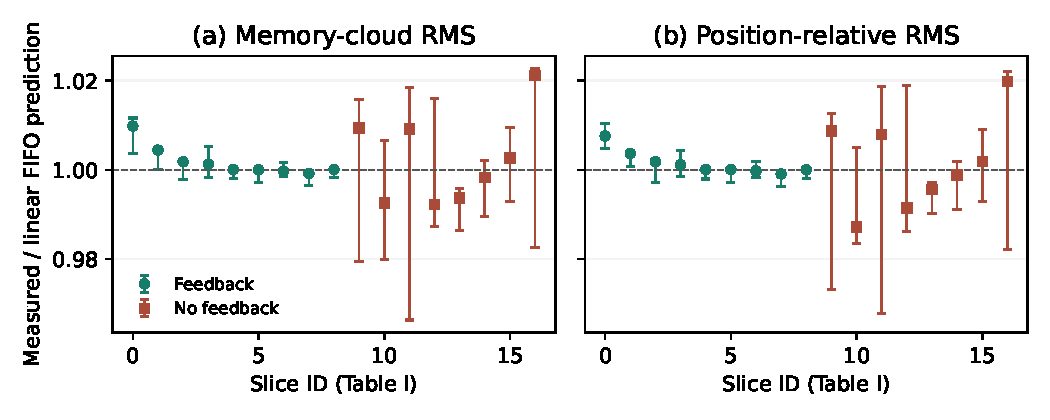
\includegraphics[width=0.96\textwidth]{../figures/matched_radius.pdf}
\caption{Observable-matched radius comparison with the linear finite-history
reference. (a) Memory-cloud RMS from the weighted trace covariance.
(b) Current-position RMS relative to the trace centroid. Symbols are
medians over five seeds, bars their IQR, and the dashed line denotes the
fixed prediction. Slice IDs and parameters appear in Table~\ref{tab:radii}.
All measurements use 10,001 terminal snapshots per seed; the earlier run
length is not the number of independent measurements.}
\label{fig:radii}
\end{figure*}

\begin{table}[tb]
\caption{Median measured/predicted RMS ratios for the archived terminal
windows. IDs 0--8 have feedback; IDs 9--16 are no-feedback controls.
Common parameters are specified in the text; ``off'' denotes $\eta=0$.}
\label{tab:radii}
\centering
\begin{tabular}{rrrrrr}
\hline\hline
ID & $d$ & $N/10^6$ & $A_a$ & $R_Q/R_{Q,H}$ & $R_r/R_{r,H}$ \\
\hline
0 & 3 & 30 & 20 & 1.0098 & 1.0076 \\
1 & 3 & 30 & 35 & 1.0045 & 1.0037 \\
2 & 4 & 30 & 35 & 1.0018 & 1.0019 \\
3 & 5 & 30 & 35 & 1.0013 & 1.0012 \\
4 & 7 & 30 & 35 & 1.0001 & 1.0001 \\
5 & 10 & 30 & 35 & 1.0000 & 1.0001 \\
6 & 13 & 30 & 35 & 0.9997 & 0.9998 \\
7 & 20 & 30 & 35 & 0.9992 & 0.9991 \\
8 & 10 & 300 & 35 & 1.0001 & 1.0000 \\
9 & 3 & 30 & off & 1.0094 & 1.0087 \\
10 & 4 & 30 & off & 0.9926 & 0.9872 \\
11 & 5 & 30 & off & 1.0092 & 1.0079 \\
12 & 7 & 30 & off & 0.9922 & 0.9914 \\
13 & 10 & 30 & off & 0.9937 & 0.9956 \\
14 & 13 & 30 & off & 0.9983 & 0.9988 \\
15 & 20 & 30 & off & 1.0027 & 1.0019 \\
16 & 10 & 300 & off & 1.0212 & 1.0198 \\
\hline\hline
\end{tabular}

\end{table}

The active memory-cloud ratios in Fig.~\ref{fig:radii}(a) have median
absolute departure $\CloudMedianError\%$ and maximum
$\CloudMaxError\%$; the corresponding position-relative departures are
$\RelativeMedianError\%$ and $\RelativeMaxError\%$.
The maximum cloud departure in the no-feedback controls is
$\ControlCloudMaxError\%$. The controls are evaluated with their own
$g=0$ reference, rather than an active-force formula.
All model coefficients come from the archived configurations. No gain,
radius, or covariance coefficient is fitted to these terminal measurements.
The comparison supports consistency with a linear relaxation cloud at these
parameters. It does not prove global confinement, a complete phase diagram,
or exact equality of the nonlinear and linear processes.

\subsection{Kernel and scale controls}
The first control compares attractive-only kernels with two-scale kernels
at equal local curvature, using $d=3$, $N=300{,}000$,
$\varepsilon=10^{-4}$, and seeds 1--5. With $s_a=3$ and $s_r=1$, the
effective amplitude of the two-scale family is
$A_{\mathrm{eff}}=A_a-9A_r$. The matched attractive-only family has
$A_a=A_{\mathrm{eff}}$, $A_r=0$.
For nine sampled positive effective amplitudes, the 45 seed-paired cloud
radius comparisons differ by at most $3.37\times10^{-6}$ relatively.
Figure~\ref{fig:controls}(a) shows the paired curves and seed IQRs.
These legacy control radii are medians of instantaneous cloud widths in
sparse traces. Both families use the same statistic, so their comparison is
valid, but these medians are not used to validate Eqs.~(\ref{eq:finite_cloud})
and (\ref{eq:estimators}). In this sampled small-radius regime, compactness
does not identify the repulsive component separately from the net curvature.

\begin{figure*}[t]
\centering
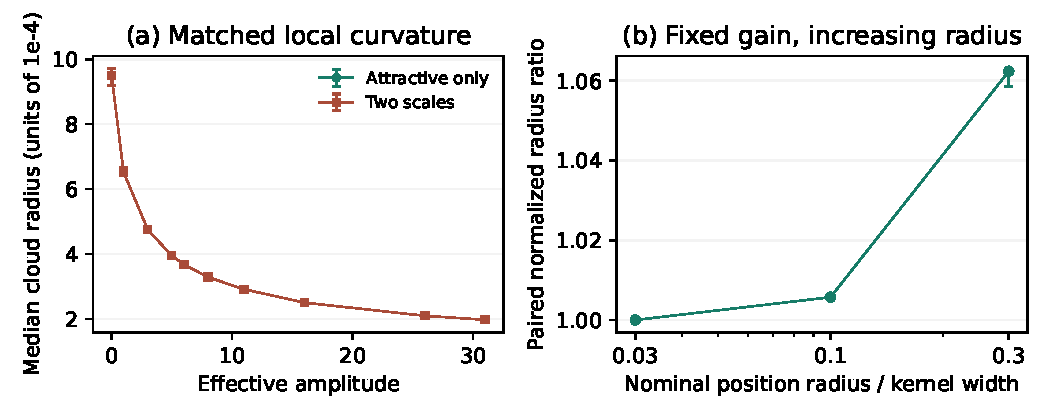
\includegraphics[width=0.96\textwidth]{../figures/kernel_controls.pdf}
\caption{Independent limits on the interpretation of compact clouds.
(a) Attractive-only and two-scale kernels matched by local curvature;
points are seed medians of the same legacy cloud-width statistic, with
seed IQRs. Their overlap tests local kernel identifiability.
(b) At fixed gain, increasing the nominal position-relative radius relative
to the kernel width yields a smooth correction. Each seed's normalized
cloud median is divided by its low-scale value before aggregation; the
endpoint median ratio is 1.0624. Bars are seed IQRs. This panel tests a
departure from scale invariance, not an absolute RMS prediction.}
\label{fig:controls}
\end{figure*}

The second control holds the attractive-only gain fixed at
$g=0.432291\ldots$ and increases the nominal position-relative
$R_r/s_a$ from 0.03 through 0.1 to 0.3 by changing $\varepsilon$.
The three amplitudes are approximately 0.04341, 0.14471, and 0.43412;
$d=3$, $N=300{,}000$, $A_a=26$, and $A_r=0$ are fixed.
The seed-paired endpoint departure in Fig.~\ref{fig:controls}(b) is
$6.24\%$. Normalization to each seed's low-scale value cancels a constant
linear conversion between cloud and position radii. The shape observables
show no coordinated transition at the sampled points. A subsequent
measurement audit found that fixed-voxel residence changed with cloud
scale, while a co-moving residence statistic saturated in both active and
no-feedback cases. The original preregistered composite classification
therefore remains \emph{inconclusive}; the post-hoc audit does not replace it.
Three sampled scales cannot exclude an unsampled bifurcation or a different
nonlinear branch.

\section{Discussion}
The simplest explanation consistent with the tested scalar branch is a
linear relative relaxation mode with a freely translating centroid.
The deposited-trace width and current-point displacement have different
stationary second moments, and comparing the correct quantities restores
agreement for both feedback and no-feedback cases. The matched-kernel
control further shows that the local curvature, rather than the detailed
two-scale structure, determines the measured compactness in the sampled
Taylor regime. The fixed-gain control identifies a smooth finite-scale
departure without isolating a metastable transition.

This evidence is limited to the archived parameters and terminal windows.
It does not establish that every realization is trapped, that the entire
nonlinear kernel has a stationary relative distribution, or that nonlinear
relative equilibria are absent elsewhere. Finite-history rotating states
are a separate deterministic question and are not needed for the present
claim. Likewise, a covariance participation dimension near $d$ is an
expected isotropic shape diagnostic in a supplied $d$-dimensional embedding;
it does not establish dimension selection.

The useful consequence is a testable baseline: evidence for a stronger
nonlinear state must depart from the observable-matched linear prediction
and survive controls with matched length and time scales. The present
results concern stochastic dynamics and measurement, without a physical
mass or spacetime interpretation.

\section*{Data and Code Availability}
The extracted terminal radius traces for all 85 seed-condition cases,
source-file hashes, configurations, numerical reference calculations,
and figure/table rebuild code are available in the versioned repository
\cite{PaperIEvidence2026}. The earlier kernel-control summaries and original
simulation code are included there. The extract contains the observables
needed for the radius analysis, not every original trajectory coordinate
or the full historical simulation output. A single script rebuilds the
reported ratios and figures without running new simulations.
